\documentclass[a4paper,10pt]{article}
\usepackage[utf8x]{inputenc}
\usepackage{amsmath}
\usepackage{graphicx}
\usepackage[english]{babel}
\usepackage{url}
\usepackage{epstopdf}
\usepackage{subfig}
\usepackage{graphicx}

\title{Procesamiento Avanzado de Imágenes\\IEE3784}
\author{\textbf{Tarea 02}\\Norman F. Sáez\\nfsaez@uc.cl}
\date{\today}

\begin{document}
\maketitle
\section{Pregunta 1}
\begin{figure}[ht!]
  \centering
  \subfloat[Cluster no supervisado:Imagen inicial]{\label{fig:img1a}\includegraphics[width=0.50\textwidth]{img/clusters.eps}}
  ~ 
  \caption{Cluster no supervisado}
  \label{fig:p1}
\end{figure}

\section{Pregunta 2}
Se pudo lograr que snakes podieran recorrer el contorno de los b-splines, con 200 iteraciones. El resultado final se puede ver en \ref{fig:p2}
\begin{figure}[ht!]
  \centering
  \subfloat[Snakes: Resultado final]{\label{fig:img2}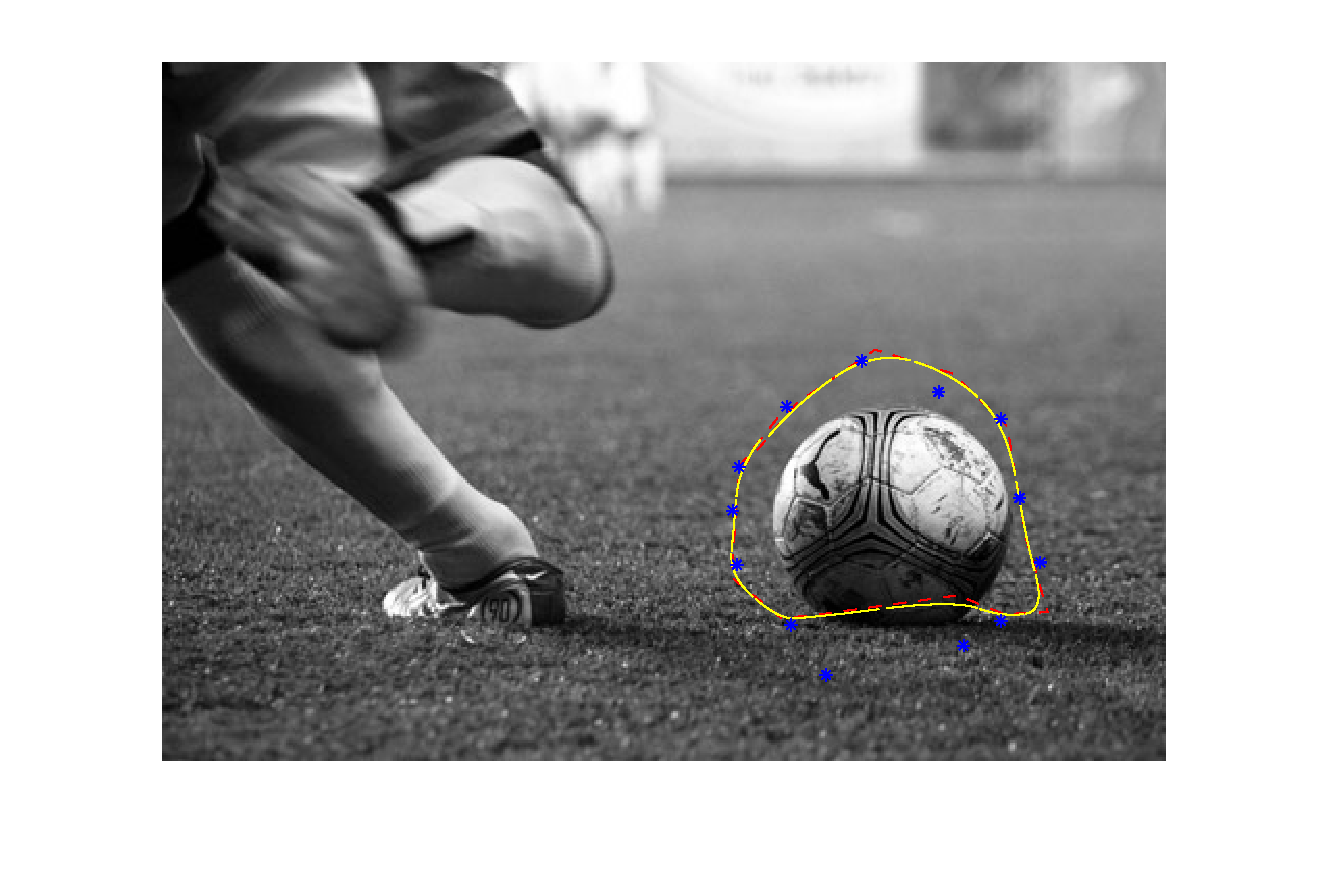
\includegraphics[width=0.80\textwidth]{img/snake_2.eps}}
  ~ 
  \caption{Azul: Puntos de control iniciales. Amarillo: b-spline.  Rojo: poligono de control}
  \label{fig:p2}
\end{figure}

Se puede decir que snakes, depende principalmente del factor viscosidad, y tambien del factor elasticidad, siendo el factor viscosidad el mas influyente en las pruebas realizadas.
\begin{figure}[ht!]
  \centering
  \subfloat[Snakes: Resultado final]{\label{fig:img22}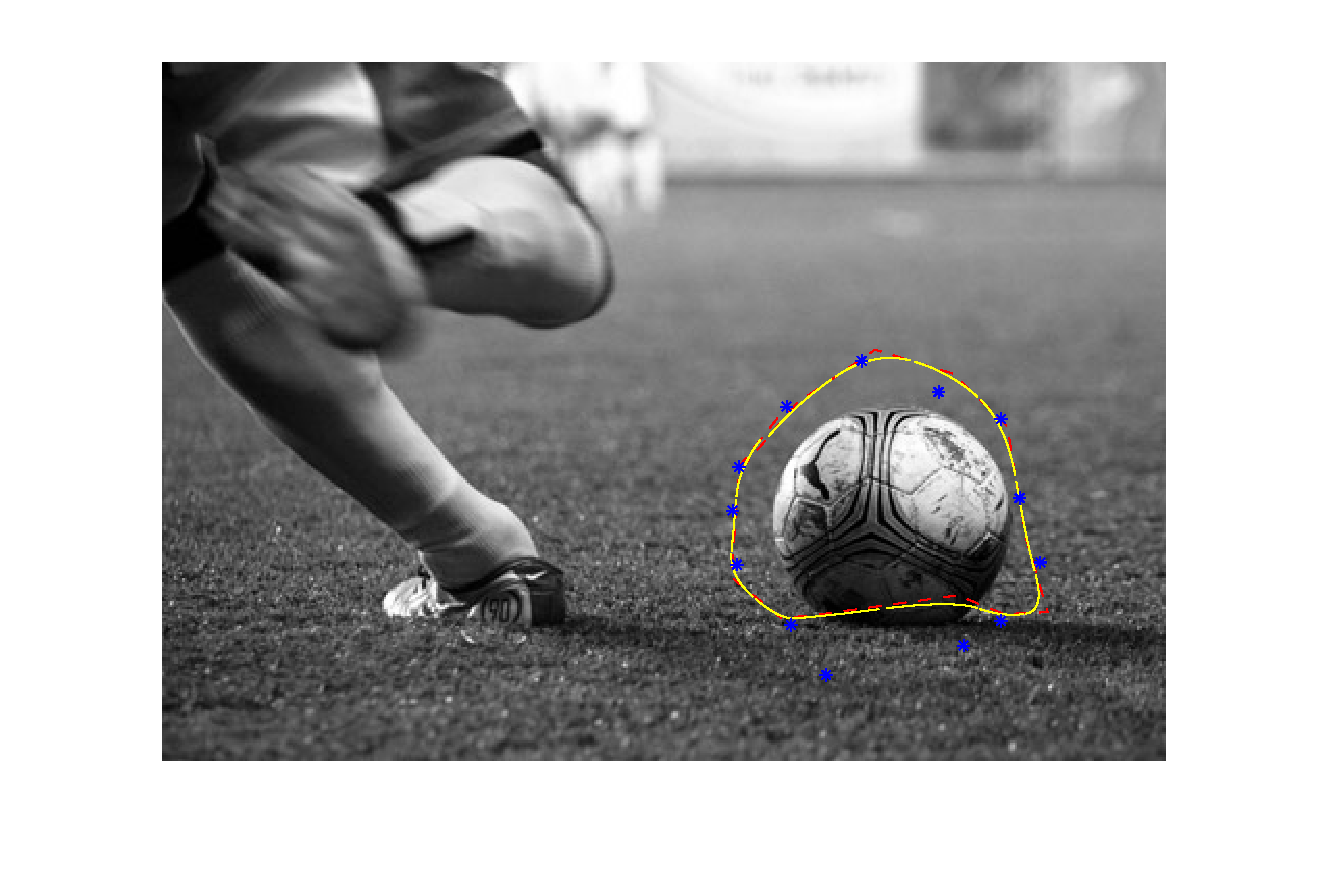
\includegraphics[width=0.50\textwidth]{img/snake_2.eps}}
  ~ 
  \subfloat[Snakes: b-spline en cada iteracion]{\label{fig:img23}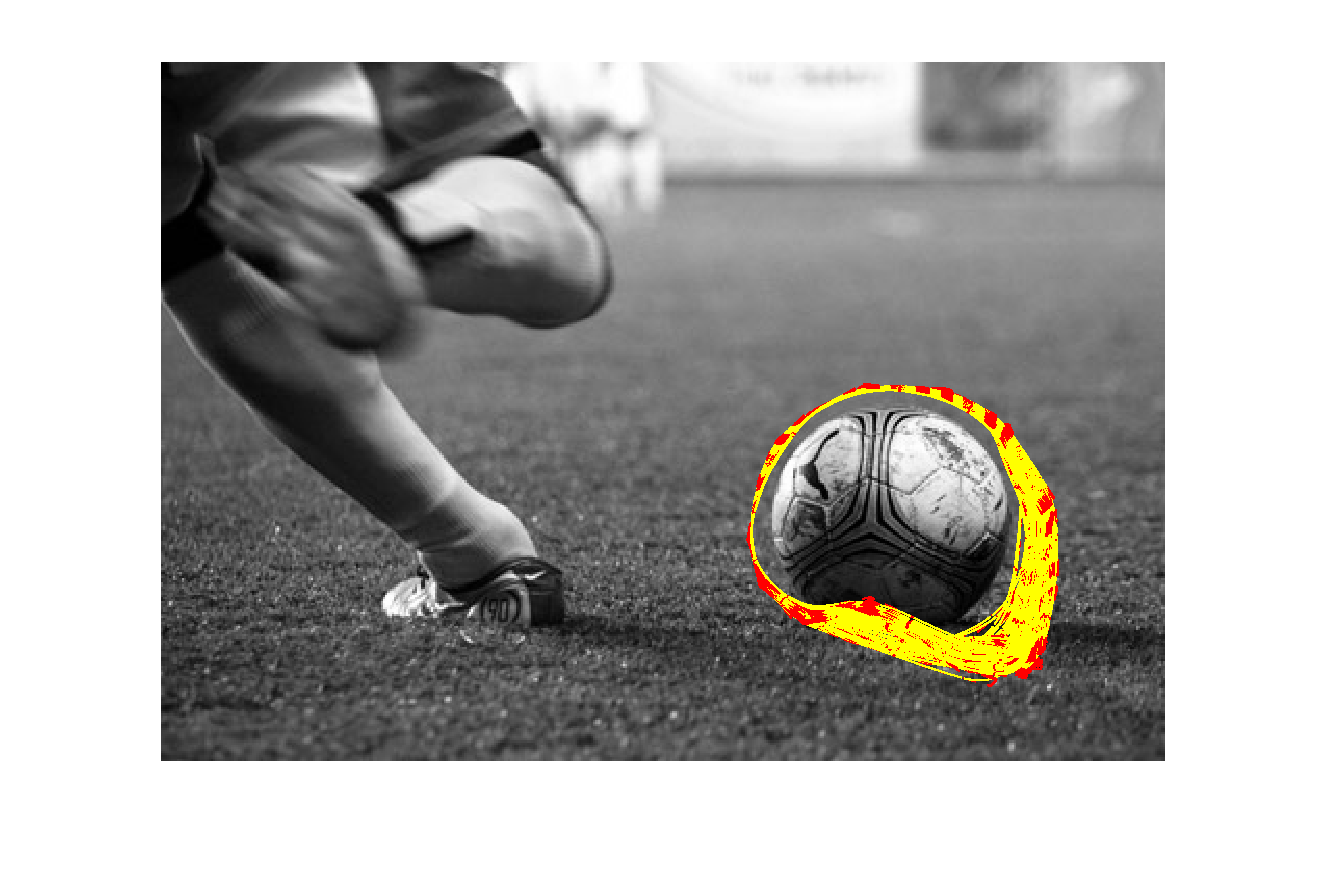
\includegraphics[width=0.50\textwidth]{img/snake_3.eps}}
  ~ 
  \caption{Azul: Puntos de control iniciales, Amarillo, b-spline, Rojo, poligono de control. }
  \label{fig:p2b}
\end{figure}
En la figura \ref{fig:p2b} se ve todas las variaciones que tuvo b-spline en cada iteracion.

\newpage
\section{Pregunta 3}
\begin{figure}[ht!]
  \centering
  \subfloat[balloons]{\label{fig:img4}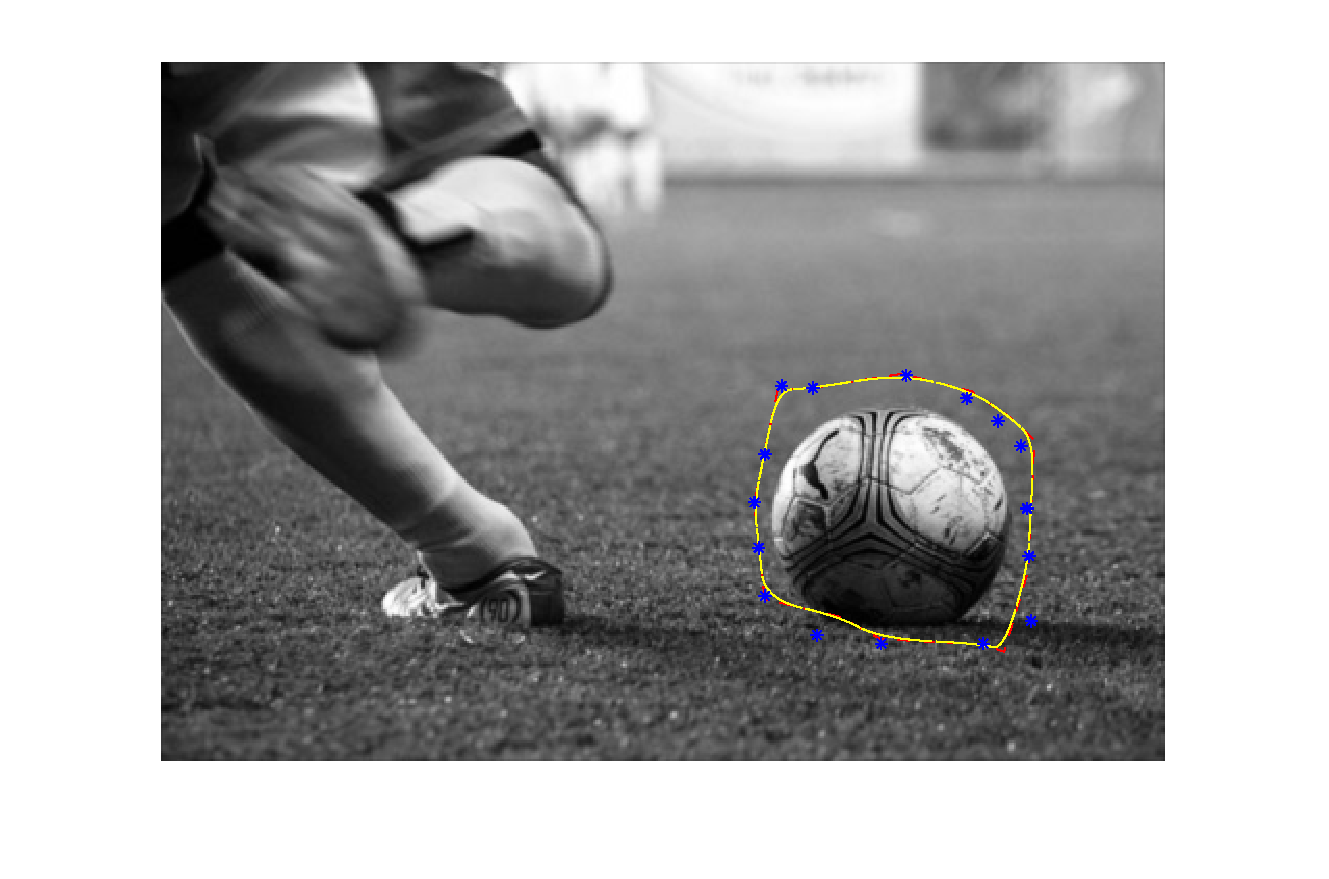
\includegraphics[width=0.50\textwidth]{img/balloon.eps}}
  ~ 
  \subfloat[balloons, con filtro gauss]{\label{fig:img4}\includegraphics[width=0.50\textwidth]{img/filtro_gauss.eps}}
  ~ 
  \caption{Ballons}
  \label{fig:p4}
\end{figure}

\end{document}
